\labday{Espaço de estado para o pêndulo não-linear}

\experiment{Resposta periódica}

Abaixo são apresentadas as figuras dos espaços de estado para frequências de forçamento que resultam em respostas periódicas.

\begin{figure}[!ht]
	\centering
	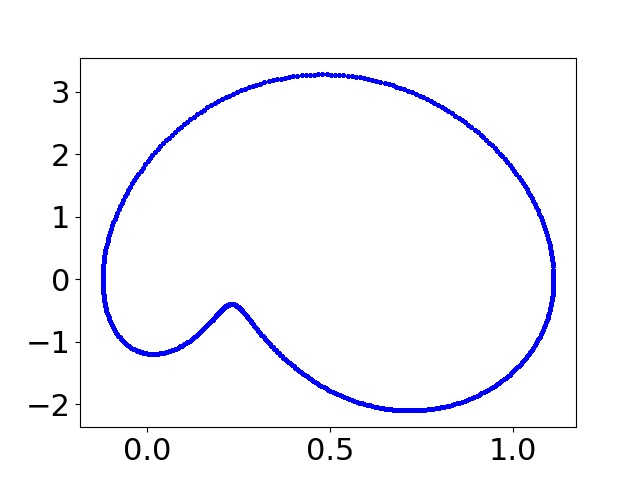
\includegraphics[scale=0.365]{state_space/figura1.jpg}
	\caption{Espaço de estado para um forçamento de 3.59 rad/s}
	\label{state_space_3.59rad/s}
\end{figure}

\begin{figure}[!ht]
	\centering
	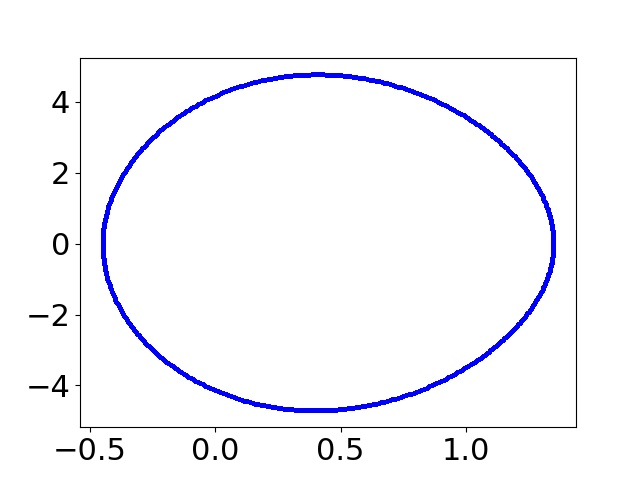
\includegraphics[scale=0.365]{state_space/figura2.jpg}
	\caption{Espaço de estado para um forçamento de 5.1 rad/s}
	\label{state_space_5.1rad/s}
\end{figure}

\experiment{Resposta caótica}

Abaixo é apresentada a figura do espaço de estado para a frequência de 5.61 $\frac{rad}{s}$, que resulta em uma resposta caótica.

\begin{figure}[!ht]
	\centering
	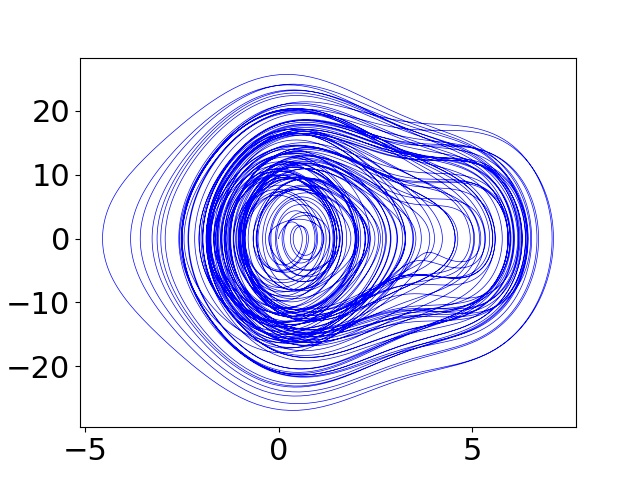
\includegraphics[scale=0.5]{state_space/figura3.jpg}
	\caption{Espaço de estado para um forçamento de 5.1 rad/s}
	\label{state_space_5.61rad/s}
\end{figure}